\documentclass{article}

\title{EFRP -  Assignment 3}
\date{2020-07-18}
\author{Marcell Granát}
% packages----------------------
\usepackage{pdfpages}
% ------------------------------
\begin{document}
  \pagenumbering{gobble}
  \maketitle
  \newpage
  
\begin{figure}[h]
  \centering
  \includegraphics[width=\textwidth]{C:/rproject/EFRP/plot/unnamed-chunk-5-1.pdf}
  \caption{fig1}
  \label{Time-series used in this study}
\end{figure}

\begin{figure}[h]
  \centering
  \includegraphics[width=\textwidth]{C:/rproject/EFRP/plot/unnamed-chunk-6-1.pdf}
  \caption{fig2}
  \label{Correlation-matrix}
\end{figure}

\begin{figure}[h]
  \centering
  \includegraphics[width=\textwidth]{C:/rproject/EFRP/plot/unnamed-chunk-8-1.pdf}
  \caption{fig3}
  \label{First difference of the time-series}
\end{figure}

\begin{figure}[h]
  \centering
  \includegraphics[width=\textwidth]{C:/rproject/EFRP/plot/unnamed-chunk-10-1.pdf}
  \caption{fig4}
  \label{Results of Engle-Granger method}
  Calculations are based on ADF-test (level, $\alpha = 5\%$)
\end{figure}

\begin{figure}[h]
  \centering
  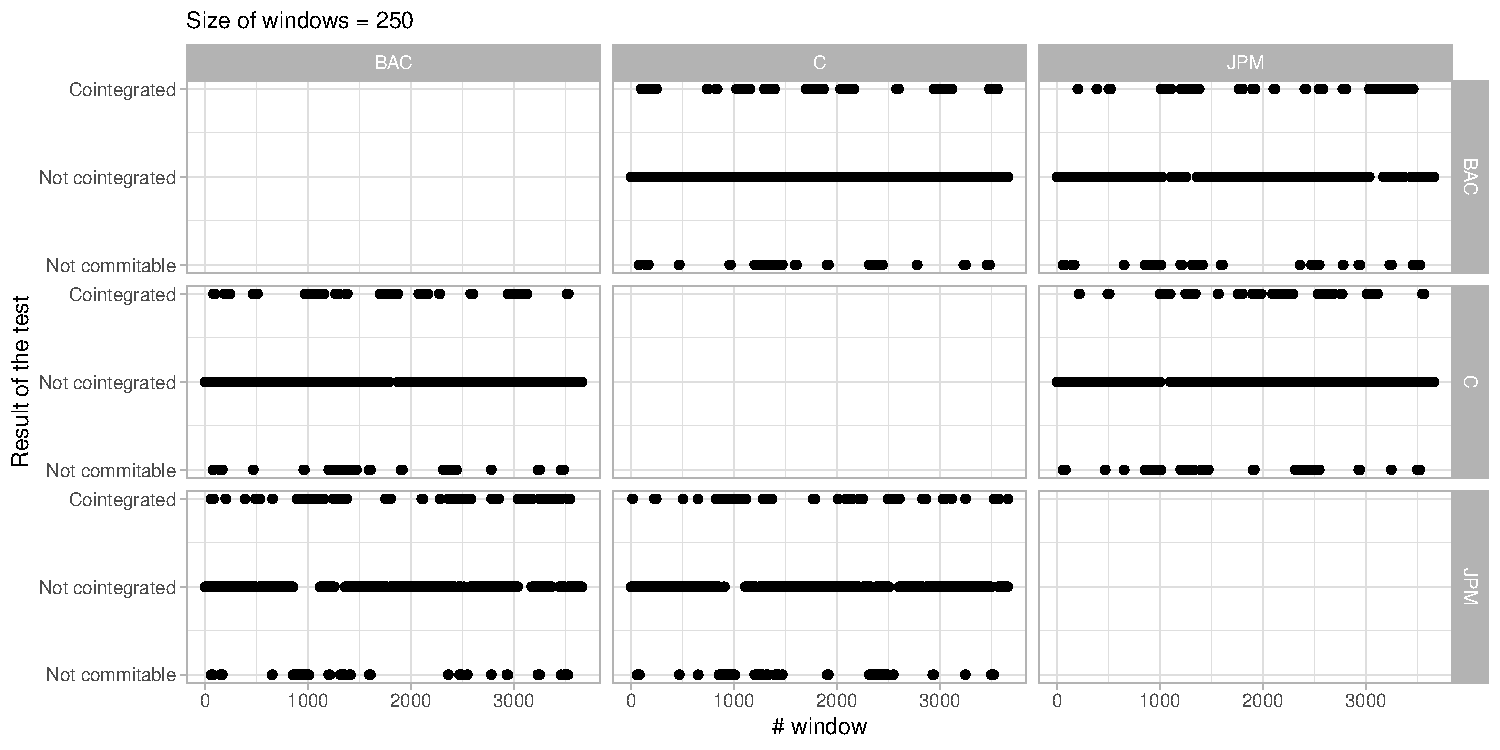
\includegraphics[width=\textwidth]{C:/rproject/EFRP/plot/unnamed-chunk-12-1.pdf}
  \caption{fig5}
  \label{Results of Engle-Granger method with rolling window}
  $Size of windows = 250$. Calculations are based on ADF-test (level, $alpha = 5\%$). Depedent variables (in the OLS) are placed horizontal, independents are vertical.
\end{figure}

\begin{figure}[h]
  \centering
  \includegraphics[width=\textwidth]{C:/rproject/EFRP/plot/unnamed-chunk-14-1.pdf}
  \caption{fig6}
  \label{Summary results of Engle-Granger method with rolling window}
  Calculations are based on ADF-test (level, $alpha = 5\%$). Number of total pairs is 6.
\end{figure}

\begin{figure}[h]
  \centering
  \includegraphics[width=\textwidth]{C:/rproject/EFRP/plot/unnamed-chunk-15-1.pdf}
  \caption{fig7}
  \label{Results of Johansen-test with rolling window across time}
  $Size of windows = 250$. Points are jittered around their true y value for better visualisation (the number of cointegrated vectors is interger). Date of recession is from the National Bureau of Economic Research (https://www.nber.org/cycles.html).
\end{figure}

\begin{figure}[h]
  \centering
  \includegraphics[width=\textwidth]{C:/rproject/EFRP/plot/unnamed-chunk-16-1.pdf}
  \caption{fig8}
  \label{Distribuiton of the Johansen-test results with rolling window}
\end{figure}

\end{document}